\chapter{Physics behind numerical methods}\label{Formulae}

\section{Distribution function transform}
Distribution function of particles in phase space is presented in code in spherical coordinates $n(\epsilon,\mu,\phi)$. Let consider transform to the frame moving along $z$-axis with lorentz-factor $\gamma = 1/\sqrt{1-\beta^2}$. Number of particles in the corresponding phase volumes $N$ is invariant.

\begin{equation}
	N = n(\epsilon,\mu,\phi)d\epsilon d\mu d\phi dV = n'(\epsilon',\mu',\phi')d\epsilon' d\mu' d\phi' dV'
\end{equation}

So, to obtain $n'$ we need to evaluate determinant of Jacobi transformation matrix. Note, that azimuthal angle phi does not changes in transformation to the moving frame $phi' = phi$, and energy and polar angle does not depend on space volume, so in general Jacobi matrix has following non-zero terms

\begin{equation}\label{generalJacobi}
	J=\left(
	\begin{array}{cccc}
		\frac{d\epsilon'}{d\epsilon} & \frac{d\epsilon'}{d\mu}& 0 & 0\\
		\frac{d\mu'}{d\epsilon} & \frac{d\mu'}{d\mu} & 0 & 0\\
		0 & 0 & 1 & 0\\
		\frac{dV'}{d\epsilon} & \frac{dV'}{d\mu} & 0 & \frac{dV'}{dV}
	\end{array}
	\right)
\end{equation}

Note, that determinant of this matrix can be decomposed by the last column and we get

\begin{equation}
|J|=\frac{dV'}{dV}\left(\frac{d\epsilon'}{d\epsilon}\frac{d\mu'}{d\mu} - \frac{d\epsilon'}{d\mu}\frac{d\mu'}{d\epsilon}\right)
\end{equation}

Let start with transforming space volume $V$. First approach, following Landau-Lifshitz 2, paragraph 10 \cite{LandauLifshitz2}, is to transform volume to the rest-frame of moving beam of particle with given momentum, and then derive that $dV'/dV= \epsilon/\epsilon'$. It is correct result, but proof is not valid for massles particles, which have not physical rest frame.

So we evaluate transformation of volume, containing chosen particles, directly from Lorentz transformations. Let assume flux of particles, aligned with z axis, with uniform interval $L$ between them, moving with same velocity $v$ with angle $\theta$ to the z axis, and $\mu = cos(\theta)$, as it is shown in Figure \ref{VolumeTransform}.

\begin{figure}[h]
	\centering
	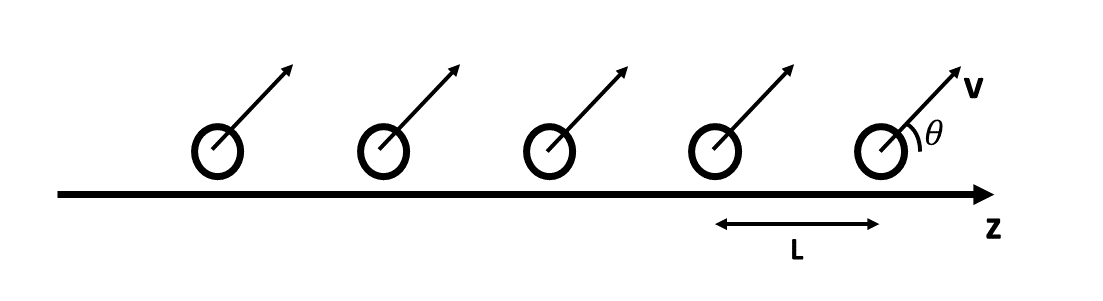
\includegraphics[width=12.5 cm]{./fig/VolumeTransform.png} 
	\caption{Beam of evenly distributed particles}
	\label{VolumeTransform}
\end{figure}

So in the lab frame, at the moment $t$ i-th particle is placed at $z_i = i\cdot L + \mu v t$. Let evaluate coordinates of particles in the moving frame.

\begin{equation}\label{lorentz_z}
	\left(\begin{array}{c}
		ct'\\
		z'_i
	\end{array}
	\right)
	= \left(
	\begin{array}{cc}
		\gamma & -\beta\gamma\\
		-\beta\gamma & \gamma
	\end{array}
	\right)
	\times
	\left(\begin{array}{c}
		ct\\
		z_i
	\end{array}
	\right)
\end{equation}

From this we can obtain values $z'_i = \gamma z_i + (\gamma \mu v - c\beta \gamma)t$, but this values are measured at the different time moments in the moving frame, if $t$ is the same for all particles in lab frame. To evaluate volume or number density we should evaluate them at the same moment $t'$. So let express $t$ in terms of $z_i$ and $t'$, and put into the equation for $z'_i$.

\begin{equation}
	t=\frac{t'+\gamma\beta z_i/c}{\gamma - \beta \mu v/c}
\end{equation}

and

\begin{equation}
	z'_i=\gamma z_i +(\gamma \mu v - c\beta \gamma)\frac{t'+\gamma\beta z_i/c}{\gamma - \beta \mu v/c}=z_i\frac{1}{\gamma(1-\beta\mu v/c)} + t'\frac{\mu v/c - \beta}{1 - \beta \mu v/c}
\end{equation}

Second term, containing $t'$ gives us standard  relativistic velocity-addition formula. And the first one gives a desired expression to the compression of the distance between particles $L' = z'_{i+1}-z'_i = L/(\gamma(1-\beta\mu v/c))$. The distances in the transversal directions does not comress with Lorentz transformations, so volume also transforms as

\begin{equation} \label{volume}
V' = V/(\gamma(1-\beta\mu v/c))
\end{equation}

This result is the same, as given by \cite{LandauLifshitz2}.

Next, we need to find expressions for $\epsilon'$ and $\mu'$, but it is better to deal with them in to separate cases - for massless and massive particles.

\subsection{Photons}
For massless photons, we consider transformation of energy-momentum vector, taking into account that $z$ component of momentum is $p_z = \mu \epsilon/c$, and transversal components stay constant.

\begin{equation}\label{lorentz_ph}
	\left(\begin{array}{c}
		\epsilon'\\
		\mu'\epsilon'
	\end{array}
	\right)
	= \left(
	\begin{array}{cc}
		\gamma & -\beta\gamma\\
		-\beta\gamma & \gamma
	\end{array}
	\right)
	\times
	\left(\begin{array}{c}
		\epsilon\\
		\mu\epsilon
	\end{array}
	\right)
\end{equation}

From the first line we get equation for Doppler shift of photon's energy

\begin{equation}\label{doppler_ph}
	\epsilon'=\gamma(1-\mu\beta)\epsilon
\end{equation}

Derivatives of $\epsilon'$ with respect to $\epsilon$ and $\mu$ are

\begin{equation}
	\frac{d\epsilon'}{d\epsilon}=\gamma(1-\mu\beta)
\end{equation}

\begin{equation}
	\frac{d\epsilon'}{d\mu}=-\gamma\beta\epsilon
\end{equation}

From the second line of \ref{lorentz_ph} we get
 $\mu'\epsilon'=-\beta\gamma\epsilon+\gamma\mu\epsilon$. Then we plug in expression for $\epsilon'$ from \ref{doppler_ph} and obtain equation for aberration of light
 
\begin{equation}\label{aberration_ph}
	\mu'=\frac{\mu-\beta}{1-\mu\beta}
\end{equation}

Angle of photon's velocity to the z-axis does not depend on their energy. And derivative of $\mu'$ with respect to $\mu$ is

\begin{equation}
	\frac{d\mu'}{d\mu} = \frac{d\mu'}{d\mu}=\frac{d}{d\mu}\frac{1}{\beta}\frac{\beta\mu-1+1-\beta^2}{1-\mu\beta}=\frac{d}{d\mu}\frac{1}{\beta}\frac{1-\beta^2}{1-\mu\beta}=\frac{1-\beta^2}{(1-\mu\beta)^2}=\frac{1}{\gamma^2(1-\mu\beta)^2}
\end{equation}

And Jacobi matrix of coordinate transformation in case of photons is

\begin{equation}
	J=\left(
	\begin{array}{cccc}
		\frac{d\epsilon'}{d\epsilon} & \frac{d\epsilon'}{d\mu}& 0 & 0\\
		0 & \frac{d\mu'}{d\mu} & 0 & 0\\
		0 & 0 & 1 & 0\\
		0 & \frac{dV'}{d\mu} & 0 & \frac{dV'}{dV}
	\end{array}
	\right)
\end{equation}

Determinant of this matrix, fortunately, equals to the multiple of diagonal terms

\begin{equation}\label{jacobian_ph}
	\frac{D(\epsilon',\mu',\phi',V')}{D(\epsilon,\mu,\phi,V)}=\frac{d\epsilon'}{d\epsilon}\frac{d\mu'}{d\mu}\frac{dV'}{dV}=\gamma(1-\mu\beta)\frac{1}{\gamma^2(1-\mu\beta)^2}\frac{1}{\gamma(1-\mu\beta)}=\frac{1}{\gamma^2(1-\mu\beta)^2}
\end{equation}

And finally, photons distribution function in spherical coordinates transforms as

\begin{equation}\label{distribution_ph}
	n'_{ph}(\epsilon',\mu',\phi') = \frac{n_{ph}(\epsilon,\mu,\phi)}{\frac{D(\epsilon',\mu',\phi',V')}{D(\epsilon,\mu,\phi,V)}}=\gamma^2(1-\mu\beta)^2 n_{ph}(\epsilon,\mu,\phi)
\end{equation}

\subsection{Massive particles}
In the case of massive particles, expression for $\epsilon'$ and $\mu'$ are more complicated. Now $p_z = \mu \sqrt{\epsilon^2 - m^2 c^4}/c$, where $m$ is particle mass, and Lorentz transformation of energy-momentum vector is expressed as

\begin{equation}\label{lorentz_m}
	\left(\begin{array}{c}
		\epsilon'\\
		\mu'\sqrt{{\epsilon'}^2 - m^2 c^4}
	\end{array}
	\right)
	= \left(
	\begin{array}{cc}
		\gamma & -\beta\gamma\\
		-\beta\gamma & \gamma
	\end{array}
	\right)
	\times
	\left(\begin{array}{c}
		\epsilon\\
		\mu\sqrt{{\epsilon}^2-m^2 c^4}
	\end{array}
	\right)
\end{equation}

So expressions for $\epsilon'$ and $\mu'$ are

\begin{equation}
	\epsilon' = \gamma\epsilon-\beta\gamma\mu\sqrt{\epsilon^2-m^2 c^4}
\end{equation}

\begin{equation}
	\mu' = \frac{-\beta\gamma\epsilon+\gamma\mu\sqrt{{\epsilon}^2-m^2 c^4}}{\sqrt{{\epsilon^2 - m^2 c^4}}}
\end{equation}

And expression for volume transformation \ref{volume} in terms of $\epsilon$ and $\mu$ is

\begin{equation}
	V'=\frac{V}{\gamma(1-\mu\beta\sqrt{{\epsilon}^2-m^2 c^4}/\epsilon)}
\end{equation}

Expressions for partial derivatives of $\epsilon'$, $\mu'$, $V'$, and especially for Jacobian are really terrible, so here we present only final result for distribution function in units $c = 1$

\begin{equation}
		\frac{n'_{m}(\epsilon',\mu',\phi')}{n_{m}(\epsilon,\mu,\phi)}= \frac{\gamma(\epsilon-\mu\sqrt{{\epsilon}^2-m^2}\beta)(\gamma^2\epsilon^2-m^2 + \mu^2 ((\epsilon^2-m^2)(\gamma^2-1)) - 2\mu\epsilon\gamma^2\beta\sqrt{\epsilon^2-m^2})^{3/2}}{\epsilon(((\gamma^2-1)(\epsilon^2-m^2)\mu^2 + \gamma^2\epsilon^2 - m^2)\sqrt{\epsilon^2-m^2}-2\mu\epsilon\gamma(\epsilon^2 - m^2)\sqrt{\gamma^2 - 1})}
\end{equation}

\section{Inverse Compton scattering}\label{comptonFormulaSection}

Consider scattering of photons on the one electron, moving along z axis, following \cite{Dubus}. Klein-Nishina cross-section in electron's rest frame is

\begin{equation}\label{KleinNishina}
	\frac{d\sigma}{d\epsilon_1'd\Omega_1'}=\frac{{r_e}^2}{2}\left(\frac{\epsilon_1'}{\epsilon_0'}\right)^2\left(\frac{\epsilon_1'}{\epsilon_0'}+\frac{\epsilon_0'}{\epsilon_1'}-\sin^2\Theta'\right) \delta\left(\epsilon_1' - \frac{\epsilon_0'}{1+\frac{\epsilon_0'}{m_e c^2}(1 - \cos \Theta')}\right)
\end{equation}

Where $r_e$ - classical electron radius, $\epsilon_0'$ and $\epsilon_1'$ - photon initial and final energies respectively $\Theta'$ angle between initial and final photon directions, defined by expression $\cos\Theta' =\cos \theta_0' \cos \theta_1' + \sin \theta_0' \sin \theta_1' \cos(\phi_1' - \phi_0')$. Primed values are measured in the electron's rest frame. Final and initial photon's energies are related as follow:

\begin{equation}
	\epsilon_1'=\frac{\epsilon_0'}{1+\frac{\epsilon_0'}{m_e c^2}(1 - \cos \Theta')}	
\end{equation}

\begin{equation}
	\epsilon_0'=\frac{\epsilon_1'}{1-\frac{\epsilon_1'}{m_e c^2}(1 - \cos \Theta')}
\end{equation}

Number of photons, which are scattered in unit solid angle in unit energy range in time unit in electron's rest frame is 

\begin{equation}
\frac{dN'}{dt'd\epsilon_1'd\Omega_1'}=\int c \frac{d\sigma}{d\epsilon_1'd\Omega_1'} \frac{dn'}{d\epsilon_0'd\Omega_0'}d\Omega_0'd\epsilon'_0
\end{equation}

Let rewrite delta-function in \ref{KleinNishina} with photon initial energy using relation

\begin{equation}
	\delta(f(x)) = \sum \frac{\delta(x-x_k)}{|f'(x_k)|}
\end{equation}

where $x_k$ - are roots of $f(x)$. Derivative of expression inside delta-function is

\begin{equation}
	\frac{d\epsilon_1'}{d\epsilon_0'}=\frac{1}{(1+\frac{\epsilon_0'}{m_e c^2}(1 - \cos \Theta'))^2}
\end{equation}

and it will cancel out with $\left(\epsilon'_1/\epsilon'_0\right)^2$ in \ref{KleinNishina}. Initial photons distribution function in the lab frame is $\frac{dn}{d \epsilon_0 d \Omega_0}$, and we transform it to the electron frame using \ref{distribution_ph}.

\begin{equation}
	\frac{dN'}{dt'd\epsilon_1'd\Omega_1'}=\int \frac{r_e^2 c}{2} \gamma_e^2 (1 - \mu_0 \beta_e)^2 \left(\frac{\epsilon_1'}{\epsilon_0'}+\frac{\epsilon_0'}{\epsilon_1'}-\sin^2\Theta'\right)\frac{dn}{d\epsilon_0 d\Omega_0} \delta\left(\epsilon_0' - \frac{\epsilon_1'}{1-\frac{\epsilon_1'}{m_e c^2}(1 - \cos \Theta')}\right) d\epsilon_0'd\mu_0' d\phi_0'
\end{equation}

Now we get rid of delta-function by integrating over $\epsilon'_0$

\begin{equation}
	\frac{dN'}{dt'd\epsilon_1'd\Omega_1'}=\int \frac{r_e^2 c}{2} \gamma_e^2 (1 - \mu_0 \beta_e)^2 \left(1 + \cos^2\Theta'+\left(\frac{\epsilon_1'}{m_e c^2}\right)^2\frac{(1-\cos\Theta')^2}{1-\frac{\epsilon_1'}{m_e c^2}(1 - \cos \Theta')}\right)\frac{dn}{d\epsilon_0 d\Omega_0}d\mu_0' d\phi_0'
\end{equation}

Now we need to transform number of scattered photons per time unit per energy unit per solid angle into the lab frame
$\frac{dN}{dt d\epsilon_1 d\Omega_1} = \frac{dN'}{dt' d\epsilon_1' d\Omega_1'}\frac{dt'}{dt}\frac{d\epsilon_1'}{d\epsilon_1}\frac{d\Omega_1'}{d\Omega_1}$. Using $dt = \gamma_e dt'$, $\epsilon = \frac{1}{\gamma_e(1 -\mu_1\beta_e)}\epsilon'$ and $\mu_1' = \frac{\mu_1-\beta_e}{1-\mu_1 \beta_e}$ we finally get

\begin{equation} \label{compton_elframe}
	\frac{dN}{dt d\epsilon_1 d\Omega_1}=\int \frac{r_e^2 c}{2} \frac{(1 - \mu_0 \beta_e)^2}{1-\mu_1\beta_e} \left(1 + \cos^2\Theta'+\left(\frac{\epsilon_1'}{m_e c^2}\right)^2\frac{(1-\cos\Theta')^2}{1-\frac{\epsilon_1'}{m_e c^2}(1 - \cos \Theta')}\right)\frac{dn}{d\epsilon_0 d\Omega_0}d\mu_0' d\phi_0'	
\end{equation}

Also it may be useful to integrate in terms of lab frame, and expression for number of scattered photons would be following
\begin{equation}\label{compton_labframe}
	\frac{dN}{dt d\epsilon_1 d\Omega_1}=\int \frac{r_e^2 c}{2} \frac{1}{\gamma_e^2(1-\mu_1\beta_e)} \left(1 + \cos^2\Theta'+\left(\frac{\epsilon_1'}{m_e c^2}\right)^2\frac{(1-\cos\Theta')^2}{1-\frac{\epsilon_1'}{m_e c^2}(1 - \cos \Theta')}\right)\frac{dn}{d\epsilon_0 d\Omega_0}d\mu_0 d\phi_0
\end{equation}

For integration one should express all angles in terms of integration variables. For evaluating photon flux from scattering on electron distribution, one should integrate formula \ref{compton_elframe} or \ref{compton_labframe} with electron distribution, normalized to the number density of particles. Note, that it is necessary to take into account different directions of electron movement, and perform corresponding rotations of coordinates.

In code compton evaluators return energy density of energy flux from the source in units of $\text{cm}^{-2} \text{s}^{-1}$. To obtain this value we perform integration of $\frac{dN}{dt d\epsilon_1 d\Omega_1}$ through the volume of the source, multiply it by energy of photon and divide by square of the distance to the source $D$.

\begin{equation}\label{comtonKlein}
	F(\epsilon_1)=\frac{\epsilon_1}{D^2}\int \frac{dN}{dt d\epsilon_1 d\Omega_1} \frac{dn_e}{d\epsilon_e d\Omega_e} dV d\epsilon_e d\Omega_e
\end{equation}

While considering processes including very high energy electrons ($\gamma_e \approx 10^8$) numerical errors can became very large, because such parameters as $\beta_e$ и $\mu_0, \mu_1, \cos \Theta'$ are very close to 1 in important energy and angle ranges, and standard type double has not enough resolution to deal with such values. So in code we introduce following auxilary variables to reduce numerical errors
:
\begin{equation}
	\delta_e = 1 - \beta_e
\end{equation}

\begin{equation}
	\text{versin}~\theta = 1 - \cos \theta
\end{equation}

Then such expression as $1 - \mu \beta_e$ with this variables can be presented as

\begin{equation}
	1 - \mu \beta_e =\text{versin}~\theta + \delta_e - \text{versin}~\theta~\delta_e
\end{equation}

and expression for angle between final and initial photons as

\begin{equation}
	1 - \cos \Theta' = \text{versin}~\theta_0' + \text{versin}~\theta_1' - \text{versin}~ \theta_0' \text{versin}~\theta_1' - \sin \theta_0'\sin \theta_1' \cos(\phi_1'-\phi_0')
\end{equation}

Use of this expressions significantly increase accuracy of numerical integration in case of high energy photons and electrons.

In case of isotropic distributionfunctions of electrons and initial photons, it is possible to integrate cross-section analytically over the angle variables \cite{JonesCompton, BykovUvarov2000}, and in the equation for enrgy flux there are only integrations by photons and electrons energy

\begin{equation}
	F(\epsilon_1)=\frac{\epsilon_1}{D^2}\int \frac{2 \pi r_e^2 \beta_e c}{\epsilon_0 \gamma_e^2} \frac{dn_{ph}}{d\epsilon_0}\frac{dn_e}{d\epsilon_e}(2 q~ \ln(q)+1+q-2q^2+\frac{q^2(1-q)\Gamma^2}{2(1+q\Gamma)})d\epsilon_0 d\epsilon_e dV
\end{equation}

where $\Gamma=4\epsilon_0\gamma_e/m_e c^2$, $q=\epsilon_1/((\gamma_e m_e c^2-\epsilon_1)\Gamma)$.

\section{Синхротронное излучение}\label{synchrotronFormulaSection}

Process of synchrotron radiation of relativistic electrons is well-known and described in classical works as for example \cite{Ginzburg1975}. But synchrotron absorption is also possible. It's cross section was obtained in \cite{Ghisellini1991}. In code we will use spectral emissivity per unit volume and absorption coefficient, described in\cite{Ghisellini}.
Emissivity (spectral density of energy radiated per unit time) per unit volume is

\begin{equation} \label{emission}
	\frac{dW(\nu)}{dt d\nu dV}=\int dE_e \frac {\sqrt {3}{e}^{3}n F(E_e) B \sin ( \phi)}{{m_e}{c}^{2}}
	\frac{\nu}{\nu_c}\int_{\frac {\nu}{\nu_c}}^{\infty }\it K_{5/3}(x)dx,
\end{equation}

where $\phi$ is angle between magnetic field and line of sight, $\displaystyle\nu_{c}$ is critical frequency defined as $\displaystyle\nu_{c} = 3 e^{2} B \sin(\phi) E^{2}/4\pi {m_{e}}^{3} c^{5}$, and~$K_{5/3}$ - Macdonald function.
Absorption coefficient for photons, propagating along line of sight is

\begin{equation}\label{absorption}
	k(\nu)=\int_{E_{min}}^{E_{max}}dE\frac {\sqrt {3}{e}^{3}}{8\pi m_e \nu^2}\frac{n B\sin(\phi)}{E^2}
	\frac{d}{dE} E^2 F(E)\frac {\nu}{ \nu_c}\int_{\frac {\nu}{ \nu_c}}^{\infty }K_{5/3}(x) dx.
\end{equation}

To evaluate observable flux in case of neglectable absorption one should integrate \ref{emission} through the volume of the source and divide result by square of the distance to the source $D$. Otherwise, one should at first solve differential equation for flux $\Phi=\frac{dW}{dt d\nu dS}$ through z direction,

\begin{equation}
\frac{d\Phi(\nu,z)}{dz} = \frac{dW(\nu)}{dt d\nu dV} - k(\nu)\Phi(\nu,z)
\end{equation}

and then integrate it through transversal directions

\begin{equation}
	F(\nu)=\frac{1}{D^2}\int dS(x,y) \Phi(\nu, x,y,z_{max})
\end{equation}

where $z_{max}$ - coordinate of surface of the source.

\subsection*{Synchrotron losses}

In case of relativistic isotropic distribution of electrons, average energy loss by one electron is described s

\begin{equation}
	\frac{dE}{dt} = -\frac{4}{3} \sigma_T c \frac{B^2}{8 \pi} \gamma_e^2
\end{equation}

where $\sigma_T$ is Thompson cross-section, and $\gamma_e$ is electron lorentz-factor. This equation can be rewritten as

\begin{equation} \label{synchlosses}
	\frac{dE}{dt} = - \frac{4}{9} \frac{e^4 B^2}{m^4 c^7} E^2
\end{equation}

Let introduce $l = \frac{4}{9} \frac{e^4 B^2}{m^4 c^7}$, so energy of particle with initial energy $E_0$ can be expressed as

\begin{equation}
	E(t) = \frac{E_0}{1 + E_0 l t}
\end{equation}

Now let evaluate how electron distribution function would change due to synchrotron losses. If initial distribution function is $F_0(E_0)$, end every particle energy losses are described with equation \ref{synchlosses}, then particles just migrate to lower energies and distribution function changes as

\begin{equation}
	F(E,t) = F_0\left(E_0(E,t)\right) dE_0/dE = F_0\left(\frac{E}{1-E l t}\right)\frac{1}{\left(1 - E l t\right)^2}
\end{equation}

If $l$ is not constant it time, then in all equations above multiple $l t$ should be replaced with $\int_0^t l(t')dt'$.

\section{Pion decay}

Two ways of evaluation spectrum of photons due to pion decay in proton-proton interactions are implemented in the code. More simple is provided by work \cite{Kelner}. Number of photons emitted in one collision is assumed to be proportional to total cross-section of inelastic p-p scattering, which is approximated as \cite{Kafexhiu}

\begin{equation}\label{sigmainel}
	\sigma_{inel} = \left(30.7 - 0.96\ln\left(E_p/E_{th}\right) + 0.18\ln^2\left(E_p/E_{th}\right) \right)\times\left(1 - \left(E_{th}/E_p\right)^{1.9}\right)^3\cdot10^{-27} \text{cm}^{2}
\end{equation}

where $E_p$ is kinetic energy of accelerated proton and $E_{th}$ is threshold kinetic energy $E_{th} = 2m_{\pi}+m^2_{\pi}/2m_p \approx 0.2797~\text{GeV}$

Number of photons emitted in energy range $\left(\epsilon, \epsilon+d\epsilon\right)$ per unit volume per unit time is

\begin{equation}
	\frac{dN}{dt d\epsilon dV} = c n_{amb} \int_{\epsilon}^{\inf}\sigma_{inel}(E_p)F(E_p)F_{\gamma}(\epsilon/E_p, E_p) dE_p/E_p
\end{equation} 

where $n_{amb}$ is number density of ambient protons, and function $F_{\gamma}(\epsilon/E_p, E_p)$ is defined as

\begin{equation}
	F_{\gamma}(x, E_p) = B \frac{\ln(x)}{x} \left(\frac{1-x^\beta}{1+k x^{\beta}\left(1-x^\beta\right)}\right)^4\times\left(\frac{1}{\ln(x)}-\frac{4\beta x^\beta}{1-x^\beta}-\frac{4 k\beta x^\beta\left(1-2x^\beta\right)}{1+k x^\beta\left(1-x^\beta\right)}\right)
\end{equation}

Parameters $B, \beta, k$ depend only on accelerated proton kinetic energy and in the energy range $0.1~\text{TeV} < E_p < 10^5~\text{TeV}$ they can be expressed as $B = 1.3 + 0.14 L + 0.011 L^2$, $\beta = 1.0/\left(1.79 + 0.11 L  + 0.008 L^2\right)$ and $k = 1.0/\left(0.801 + 0.049 L + 0.014 L^2\right)$, where $L = \ln\left(E_p/1~\text{TeV}\right)$

In more complicated model, described in \cite{Kafexhiu} direct cross-sections of pion producing in proton-proton scatetering are used at low energies ($E_p < 2~\text{GeV}$), while at high energy number of emitted photons is evaluated with similar approach using $\sigma_{inel}$, but with more accurate correction coefficients.

At low energies the cross-section of producing pion $\sigma_{\pi}$ is sum of cross-sections of three processes - with producing one pion $pp\rightarrow pp\pi^0$ and with producing two pions $pp\rightarrow pp2\pi^0$ and $pp\rightarrow \{pn,D\}\pi^{+}\pi^0$. The first one has cross-section

\begin{equation}
	\sigma_{1\pi} = 7.66\times10^{-30}\eta^{1.95}\left(1 + \eta + \eta^5\right)\times\left(f_{BW}\left(\sqrt s\right)\right)^{1.86}~\text{cm}^{2}
\end{equation}

where $s = 2 m_p \left(E_p+2m_p\right)$ is square of energy in center-mass frame and $\eta$ is normalized maximal pion momentum

\begin{equation}
	\eta = \frac{\sqrt{\left(s-m_{\pi}^2-4m_p^2\right)^2-16 m_{\pi}^2m_p^2}}{2m_{\pi}\sqrt{s}}
\end{equation}

and $f_{BW}$ is the relativistic Breight-Wigner distribution

\begin{equation}
	f_{BW}\left(\sqrt{s}\right)=\frac{m_p K}{\left(\left(\sqrt{s}-m_p\right)^2-M_{res}^2\right)^2+M_{res}^2\Gamma_{res}^2}
\end{equation}

where $K = \sqrt{8}M_{res}\Gamma_{res}\gamma/\pi\sqrt{M_{res}^2+\gamma}$ and $\gamma = \sqrt{M_{res}^2\left(M_{res}^2+\Gamma_{res}^2\right)}$. The values of parameters are $M_{res} = 1.1883~\text{GeV}$ and $\Gamma_{res} = 0.2264~\text{GeV}$.

The combined cross section of processes, producing two pions is

\begin{equation}
	\sigma_{2\pi}=\frac{5.7\cdot10^{-27}}{1+\exp(-9.3\left(E_p/1~\text{GeV} - 1.4\right))}
\end{equation}

for energies $E_p > 0.56~\text{GeV}$ and for lower energies $\sigma_{2\pi}=0$.

For energies above 2 GeV, cross-section of pion producing is evaluate using average number of produced pions in one collision and total inelastic cross-section \ref{sigmainel} $\sigma_{\pi} = \braket{n_{\pi}} \sigma_{inel}$. For energies above 1 GeV and below 5 GeV $\braket{n_{\pi}} = -0.006 + 0.237 Q - 0.023 Q^2$ where $Q = \left(E_p - E_{th}\right)/m_p$. And for energies above 5 GeV average number of produced pions is $\braket{n_{\pi}} = a_1 \xi^{a_4}\left(1 + \exp\left(-a_2\xi^{a_5}\right)\right)\left(1-\exp\left(-a_3\xi^{1/4}\right)\right)$, where $\xi = \left(E_p/1~\text{GeV} - 3\right)/m_p$ and coefficients $a_1-a_5$ are obtained with numerical simulations with GEANT code \cite{AllisonGeant2006}, $a_1 = 0.728, a_2 = 0.596, a_3 = 0.491, a_4 = 0.2503, a_5 = 0.117$.

Now, having $\sigma_{\pi}$, cross-section of emitting photon in energy range $\left(\epsilon, \epsilon + d\epsilon\right)$ can be expressed as follow

\begin{equation}
	\frac{d\sigma_{\gamma}\left(E_p, \epsilon\right)}{d\epsilon} = A_{max}\left(E_p\right)\times F\left(E_p, \epsilon\right)
\end{equation}

where $A_{max}(E_p)$ is a maximum cross-section for all photons energies, so it depends only on proton energy, and $F\left(E_p,\epsilon\right)$ describes photon spectrum. To write expression for $F\left(E_p, \epsilon\right)$ one need to introduce variable, describing kinematics first. $Y=\epsilon+\frac{m_{\pi}^2}{4 \epsilon}$, $Y_{max}=\epsilon_{max}+\frac{m_{\pi}^2}{4 \epsilon_{max}}$, where $\epsilon_{max}$ is the maximum photon energy possible for given proton energy, $X=\frac{Y-m_{\pi}}{Y_{max}-m_{\pi}}$. Energy of pion in center-mass frame is $E_{CM}=\frac{s-4m_p^2+m_{\pi}^2}{s\sqrt{s}}$ and maximum pion energy in labaratory frame is $E_{max}=\gamma_{CM}\left(E_{CM}+\sqrt{E_{CM}-m_{\pi}^2}\beta_{CM}\right)$, where lorentz-factor of center-mass frame is $\gamma_{CM}=\frac{E_p+2m_p}{\sqrt{s}}$ and $\beta_{CM}=\sqrt{1-1/\gamma_{CM}^2}$. Now formula for $F\left(E_p,\epsilon\right)$ is
\begin{equation}
	F\left(E_p,\epsilon\right) = \frac{\left(1-X^{\alpha(E_p)}\right)^{\beta(E_p)}}{\left(1+X Y_{max}/\lambda m_{\pi}\right)^{\gamma(E_p)}}
\end{equation}

Exact expressions for $\lambda, \alpha(E_p), \beta(E_p), \gamma(E_p)$ are described in \cite{Kafexhiu}.

And finally $A_{max}$ can be expressed as $5.9\times\frac{\sigma_{\pi}}{E_{max}}$ for proton energies < 1 GeV, and as $b_1 \left(E_p/m_p\right)^{-b_2}\exp\left(b_3 \ln^2\left(E_p/m_p\right)\right)\times\frac{\sigma_{\pi}}{m_p}$ for higher energies. Expressions for $b_1, b_2, b_3$ also can be found in \cite{Kafexhiu}. The total number of emitted photons per unit time per unit energy in energy range $\left(\epsilon, \epsilon + d\epsilon\right)$ can be found by integrating $\frac{d\sigma_{\gamma}\left(E_p, \epsilon\right)}{d\epsilon}$ with accelerated protons distribution

\begin{equation}
	\frac{dN}{dt d\epsilon dV} = c n_{amb} \int_{\epsilon}^{\inf}\frac{d\sigma_{\gamma}\left(E_p, \epsilon\right)}{d\epsilon} F(E_p) dE_p
\end{equation} 

\section{Bremsstrahlung}

For simple case bremssrahlung from thermal not relativistic plasma, we use equations provided by \cite{Rybicki}. Amount of energy, emitted per unit energy per unit time per unit volume is

\begin{equation}
	\frac{dW}{dt d\epsilon dV} = \frac{2^5 \pi e^6}{3 h m c^3}\sqrt{\frac{2\pi}{3 k m}}T^{-1/2}Z^2n_e n_i\exp\left(-\frac{\epsilon}{kT}\right)\bar{G}
\end{equation}

where $T$ is plasma temperature, $n_e, n_i$ are electron and ion concentrations respectively, $Z$ is charge number of ions and $\bar{G}$ is velocity averaged gaunt factor. Approximate formulas for $\bar{G}$ are provided by Novikov and Thorne \cite{NovikovThorne} and corrected by Rybicki and Lightman \cite{Rybicki}. Formulas for different scattering regimes - for small-angle and, large-angle scattering, and also for classical, and for regime when quantum effects and uncertainty principle (U.P.) is important, are shown in Figure \ref{gaunt}, where $R_y$ is Rydberg constant and $\xi$ is Euler-Mascheroni constant.

\begin{figure}
	\centering
	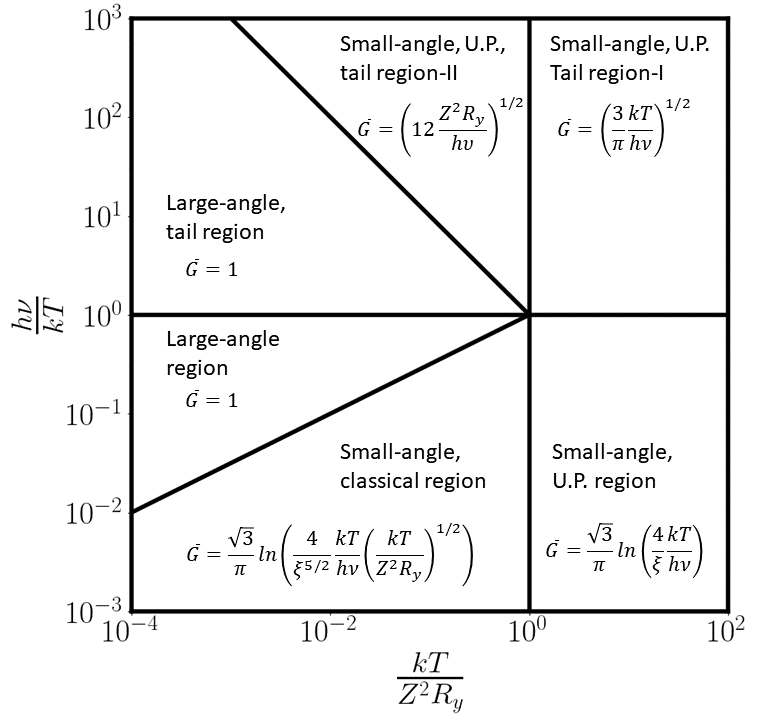
\includegraphics[width=11.5 cm]{./fig_en/gaunt.png} 
	\caption{Gaunt factor from Rybicki and Lightman \cite{Rybicki} (corrected), originally from Novikov and Thorne \cite{NovikovThorne}}
	\label{gaunt}
\end{figure}

For case of general isotropic distributions of electrons we use approach described in \cite{Baring1999}. Number of emitted photons per unit energy per unit time per unit volume by electons distribution is

\begin{equation}
	\frac{dN}{dt d\epsilon dV} = \int\frac{dN_{\gamma}\left(E_e, \epsilon\right)}{dt d\epsilon} F(E_e) dE_e
\end{equation}

where $\frac{dN_{\gamma}\left(E_e, \epsilon\right)}{dt d\epsilon}$ is number of photons emitted by single electron with energy $E_e$. It is defined by equation

\begin{equation}
	\frac{dN_{\gamma}\left(E_e, \epsilon\right)}{dt d\epsilon} = v_e \left(\left(\sum n_i Z_i^2\right)\sigma_{e-p} + n_e\sigma_{e-e}\right)
\end{equation}

where $v_e$ is electron velocity, $n_i, Z_i$ are number density and charge number of each ion species, and $\sigma_{e-p}$ and $\sigma_{e-e}$ are electron-proton and electron-electron scattering cross-sections respectively.

Electron-electron cross-section for relativistic regime ($E_e > 2~\text{MeV}$) can be expressed in following form, derived in \cite{BaierJETP1967} : $\sigma_{e-e}(E_e,\epsilon) = \left(\sigma_1 + \sigma_2\right)A\left(\epsilon, E_e/m_e c^2\right)$, and

\begin{equation}\label{sigma1}
	\sigma_1 = \frac{4 r_e^2 \alpha}{\epsilon}\left(1+\left(\frac{1}{3}-\frac{\epsilon}{\gamma_e}\right)\left(1-\frac{\epsilon}{\gamma_e}\right)\right)\left(\ln\left(2\gamma_e\frac{\gamma_e - \epsilon}{\epsilon}\right)-\frac{1}{2}\right)
\end{equation}

while expression for $\sigma_2$ is splitted into two cases. For $\epsilon < 1/2$ it is

\begin{equation}
	\begin{split}
	\sigma_2 = \frac{r_e^2\alpha}{3\epsilon} \left( 16 \left( 1-\epsilon+\epsilon^2 \right) \ln\frac{\gamma_e}{\epsilon}-\frac{1}{\epsilon^2}+\frac{3}{\epsilon}-4+4\epsilon-8\epsilon^2 \right. \\ \left. - 2\left( 1-2\epsilon \right) \ln \left( 1-2\epsilon \right) \left( \frac{1}{4\epsilon^3}-\frac{1}{2\epsilon^2}+\frac{3}{\epsilon}-2+4\epsilon \right) \right)
	\end{split}
\end{equation}

and for $\epsilon > 1/2$

\begin{equation}
	\sigma_2 = \frac{r_e^2\alpha}{3\epsilon}\frac{2}{\epsilon}\left(\left(4-\frac{1}{\epsilon}+\frac{1}{4\epsilon^2}\right)\ln\left(2\gamma_e\right)-2+\frac{2}{\epsilon}-\frac{5}{8\epsilon^2}\right)
\end{equation}

where $r_e$ is classical electro nradius and $\alpha$ is the fine structure constant. Correction factor $A(\epsilon, \gamma_e)$ is

\begin{equation}
	A\left(\epsilon, \gamma_e\right)=1-\frac{8}{3}\frac{\left(\gamma_e-1\right)^5}{\gamma_e + 1}\left(\frac{\epsilon}{\gamma_e}\right)^{1/3}
\end{equation}

In not relativistic regime, electron-electron scattering cross-section is 

\begin{equation}
	\sigma_{NR}=\frac{4r_e^2\alpha}{15\epsilon}F\left(\frac{4\epsilon}{\gamma_e^2-1}\right)
\end{equation}

where

\begin{equation}
	\begin{split}
	F(x) = \left(1+\frac{1}{2}\left(\gamma_e^2-1\right)\right)\left(17-\frac{3x^2}{\left(2-x\right)^2}-\frac{10x\gamma_e\beta_e\left(2+\gamma_e\beta_e\right)}{1+x^2\left(\gamma_e^2-1\right)}\right)\sqrt{1-x} \\ +\left(12\left(2-x\right)-\frac{7x^2}{2-x}-\frac{3x^4}{\left(2-x\right)^3}\right)\ln\frac{1+\sqrt{1-x}}{\sqrt{x}}
	\end{split}
\end{equation}

Cross-section for electron-proton scattering is provided by Bethe and Heitler \cite{BetheHeitler}. Note, that in the ultrarelativistic electron it is equal to $\sigma_1$ \ref{sigma1} \cite{JauchRohrlich}. In general, Bethe-Heitler cross-section is

\begin{equation}
	\begin{split}
	\sigma_{e-p} = \frac{r_e^2\alpha}{\epsilon}\frac{p'}{p}\left(\frac{4}{3}-\frac{2}{\left(\beta_e\beta_e'\right)^2}\left(\frac{\gamma_e}{\gamma_e'}+\frac{\gamma_e'}{\gamma_e}-\frac{2}{\gamma_e\gamma_e'}\right) + \right. \\ \left. \left(l\frac{\gamma_e'}{\gamma_e^2-1}+l'\frac{\gamma_e}{\gamma_e'^2-1}-l l'\right) + L\left(\frac{8}{3}\gamma_e\gamma_e'+\epsilon^2\left(\frac{1}{\left(\beta_e\beta_e'\right)^2+1}\right)+ \right. \right. \\ \left. \left. \frac{1}{2}\epsilon\left(l\left(1+\frac{\gamma_e'}{\beta_e^2\gamma_e}\right)-l'\left(1+\frac{\gamma_e}{\beta_e'^2\gamma_e'}\right)+2\frac{\epsilon}{\beta_e^2\gamma_e\beta_e'^2\gamma_e'}\right)\right)\right)
	\end{split}
\end{equation}

Following notations are used: $\gamma_e$ - lorentz-factor of initial electron, $\beta_e$ - it's unitless velocity, $l = \frac{1}{\beta_e\gamma_e}\ln\frac{1+\beta_e}{1-\beta_e}$, primed values are related to scattered electron and $\gamma_e = \gamma_e' + \epsilon$. And finally $L = \frac{2}{\beta_e\gamma_e\beta_e'\gamma_e'}\ln\frac{\gamma_e\gamma_e'\left(1+\beta_e\beta_e'\right)-1}{\epsilon}$.